% Unofficial University of Cambridge Poster Template
% https://github.com/andiac/gemini-cam
% a fork of https://github.com/anishathalye/gemini
% also refer to https://github.com/k4rtik/uchicago-poster

\documentclass[final]{beamer}

% ====================
% Packages
% ====================

\usepackage[T1]{fontenc}
\usepackage{lmodern}
\usepackage[orientation=portrait,size=a0,scale=1.25]{beamerposter}
\usetheme{gemini}
\usecolortheme{nott}
\usepackage{graphicx}
\usepackage{booktabs}
\usepackage{tikz}
\usepackage{pgfplots}
\pgfplotsset{compat=1.14}
\usepackage{anyfontsize}

% for tables
\usepackage{multirow}
\usepackage{multicol}
\usepackage{transparent}

% for urls
\usepackage{hyperref}

% for subfigures
\usepackage{caption}
\usepackage{subcaption}

% for bibliography
\renewcommand{\refname}{Literature}
\usepackage[backend=biber]{biblatex}
\addbibresource{../presentation/references.bib}

% for inline code listings
\usepackage{listings}
\usepackage{xparse}
\usepackage{xcolor}
\definecolor{codeblue}{rgb}{0.0, 0.0, 1.0}
\definecolor{codegreen}{rgb}{0.0, 0.5, 0.0}
\definecolor{codegray}{rgb}{0.5, 0.5, 0.5}
\definecolor{codepurple}{rgb}{0.58, 0.0, 0.82}
\definecolor{backcolour}{rgb}{0.95, 0.95, 0.92}
\lstdefinestyle{py}{
    language=Python,
    %  backgroundcolor=\color{backcolour},
    commentstyle=\color{codegreen},
    keywordstyle=\color{codeblue},
    numberstyle=\tiny\color{codegray},
    stringstyle=\color{codepurple},
    basicstyle=\small\ttfamily,
    breakatwhitespace=false,
    breaklines=true,
    captionpos=b,
    keepspaces=true,
    numbers=left,
    numbersep=5pt,
    showspaces=false,
    showstringspaces=false,
    showtabs=false,
    tabsize=4,
    frame=0,
    rulecolor=\color{black},
    morekeywords={self, assert, yield, None, True, False}
}

% ====================
% Lengths
% ====================

% If you have N columns, choose \sepwidth and \colwidth such that
% (N+1)*\sepwidth + N*\colwidth = \paperwidth
\newlength{\sepwidth}
\newlength{\colwidth}
\setlength{\sepwidth}{0.025\paperwidth}
\setlength{\colwidth}{0.45\paperwidth}

\newcommand{\separatorcolumn}{\begin{column}{\sepwidth}\end{column}}

% ====================
% Title
% ====================

% Title page
\title{\Large Network Diffusion --- Framework to Simulate Spreading Processes in Complex Networks}
\author{\large
    \textbf{Micha{\l} Czuba} \inst{1},
    Mateusz Nurek \inst{1},
    Damian Serwata \inst{1},
    Yu-Xuan Qi \inst{2},
    Mingshan Jia \inst{2},
    Katarzyna Musial \inst{2},
    Rados{\l}aw Michalski \inst{1},
    Piotr Br{\'o}dka \inst{1}
}
\institute{
  \inst{1} Wroc{\l}aw University of Science and Technology, PL, EU\\
  \inst{2} University of Technology Sydney, NSW, AU
}

% ====================
% Footer (optional)
% ====================

\footercontent{
  \href{https://networks.pwr.edu.pl/}{https://networks.pwr.edu.pl} \hfill
  NetSci, Canada, June 2024 \hfill
  \href{mailto:michal.czuba@pwr.edu.pl}{michal.czuba@pwr.edu.pl}}

% ====================
% Logo (optional)
% ====================

\logoright{
\includegraphics[height=4cm]{logos/nsl-white.pdf}}
\logoleft{
\includegraphics[height=4cm]{logos/wust_logo.pdf}}

% ====================
% Body
% ====================

\begin{document}

\begin{frame}[t, fragile]
\begin{columns}[t]

\separatorcolumn
\begin{column}{\colwidth}

\begin{block}{Introduction}
    Spreading phenomena are one of the issues considered by network science. They can be observed in
    various areas, such as dynamics of political opinions, marketing campaigns, spread of epidemics,
    etc. With the advancement of network science, analytical approaches have become insufficient for
    large graphs, prompting researchers to use computational methods. Moreover, recent years brought
    a significant expansion of the scope of network science beyond static graphs to encompass more
    complex structures. The introduction of streaming, temporal, multilayer, and hypernetwork
    approaches has brought new possibilities and imposed additional requirements. Unfortunately, the
    pace of advancement is often too rapid for existing computational packages to keep up with the
    functionality updates.
\end{block}

\begin{block}{Problem}
    There are many very good and efficient tools that help in simulating diffusion processes in
    networks, e.g. \lstinline[style=py]{ndlib} (which we love). \\
    \vspace{2em}
    However, if we consider...\\
    \vspace{1em}
    \hspace{5em}...more complex network models,... \\
    \vspace{1em}
    \hspace{5em}...spreading multiple processes at the same time... \\
    \vspace{1em}
    \hspace{14em}...\textbf{a gap among the available toolkits} emerges.
\end{block}

\begin{alertblock}{Our Contribution}
    In order to address the issue, we decided to redesign, polish, and share the simulation 
    environment we are internally using in the lab. Thus, in our recent
    work~\cite{czuba2024networkdiffusion}, we presented \lstinline[style=py]{network-diffusion}.
    To start using the library, just type in your shell:
    \begin{center}
        \large
        \begin{verbatim}
            pip install network-diffusion
        \end{verbatim}
    \end{center}
    \vspace{-1em}
    Or scan this QR code to reach the docs with more examples:
    \begin{figure}
        
\includegraphics[width=15cm]{../presentation/figures/qr_code2.pdf}
    \end{figure}
\end{alertblock}

\begin{block}{Key Features of \lstinline[style=py, basicstyle=\large\ttfamily]{network-diffusion}}
    \begin{itemize}
        \item \textbf{End-to-End Simulation Workflow for Discrete Diffusion Phenomena}
        \item \textbf{Support for Temporal Network Models}
        \item \textbf{Support for Multilayer Network Models}
        \item \textbf{A Bunch of Predefined Spreading Models}
        \item \textbf{An Interface for Implementing Custom Spreading Models}
        \item \textbf{New Centrality Measures}
        \item \textbf{\lstinline[style=py, basicstyle=\large\ttfamily]{networkx} Compatibility}
    \end{itemize}
\end{block}

\begin{exampleblock}{Example}
    \heading{Linear Threshold Model in Multilayer Networks}
    In a diffusion under the Linear Threshold Model (LTM), each node:
    \begin{itemize}
        \item can fall in two states: \textit{active} and \textit{inactive},
        \item becomes \textit{active} if the fraction of its \textit{active} neighbors to all 
        neighbours exceeds a certain threshold ($\mu$).
    \end{itemize}
    In the case of multilayer networks --- actors are the subject of the process, while the 
    nodes are their auxiliary representation. Thus, we have to define how to aggregate impulses 
    from the layers. In this example, we will consider $OR$ strategy (aka protocol), which says that
    the actor can be activated if any of the nodes representing it gets activated.
\end{exampleblock}

\end{column}

\separatorcolumn
\begin{column}{\colwidth}

\begin{exampleblock}{Example}

\heading{Scenario to Simulate}
The Figure below shows the case we would like to model with \lstinline[style=py]{network-diffusion} 
--- mLTM with homogeneous threshold $\mu=0.3$ and protocol $OR$. The process will diffuse in a
network with eleven actors, starting from the agents six and ten.
\begin{figure}
    \centering
    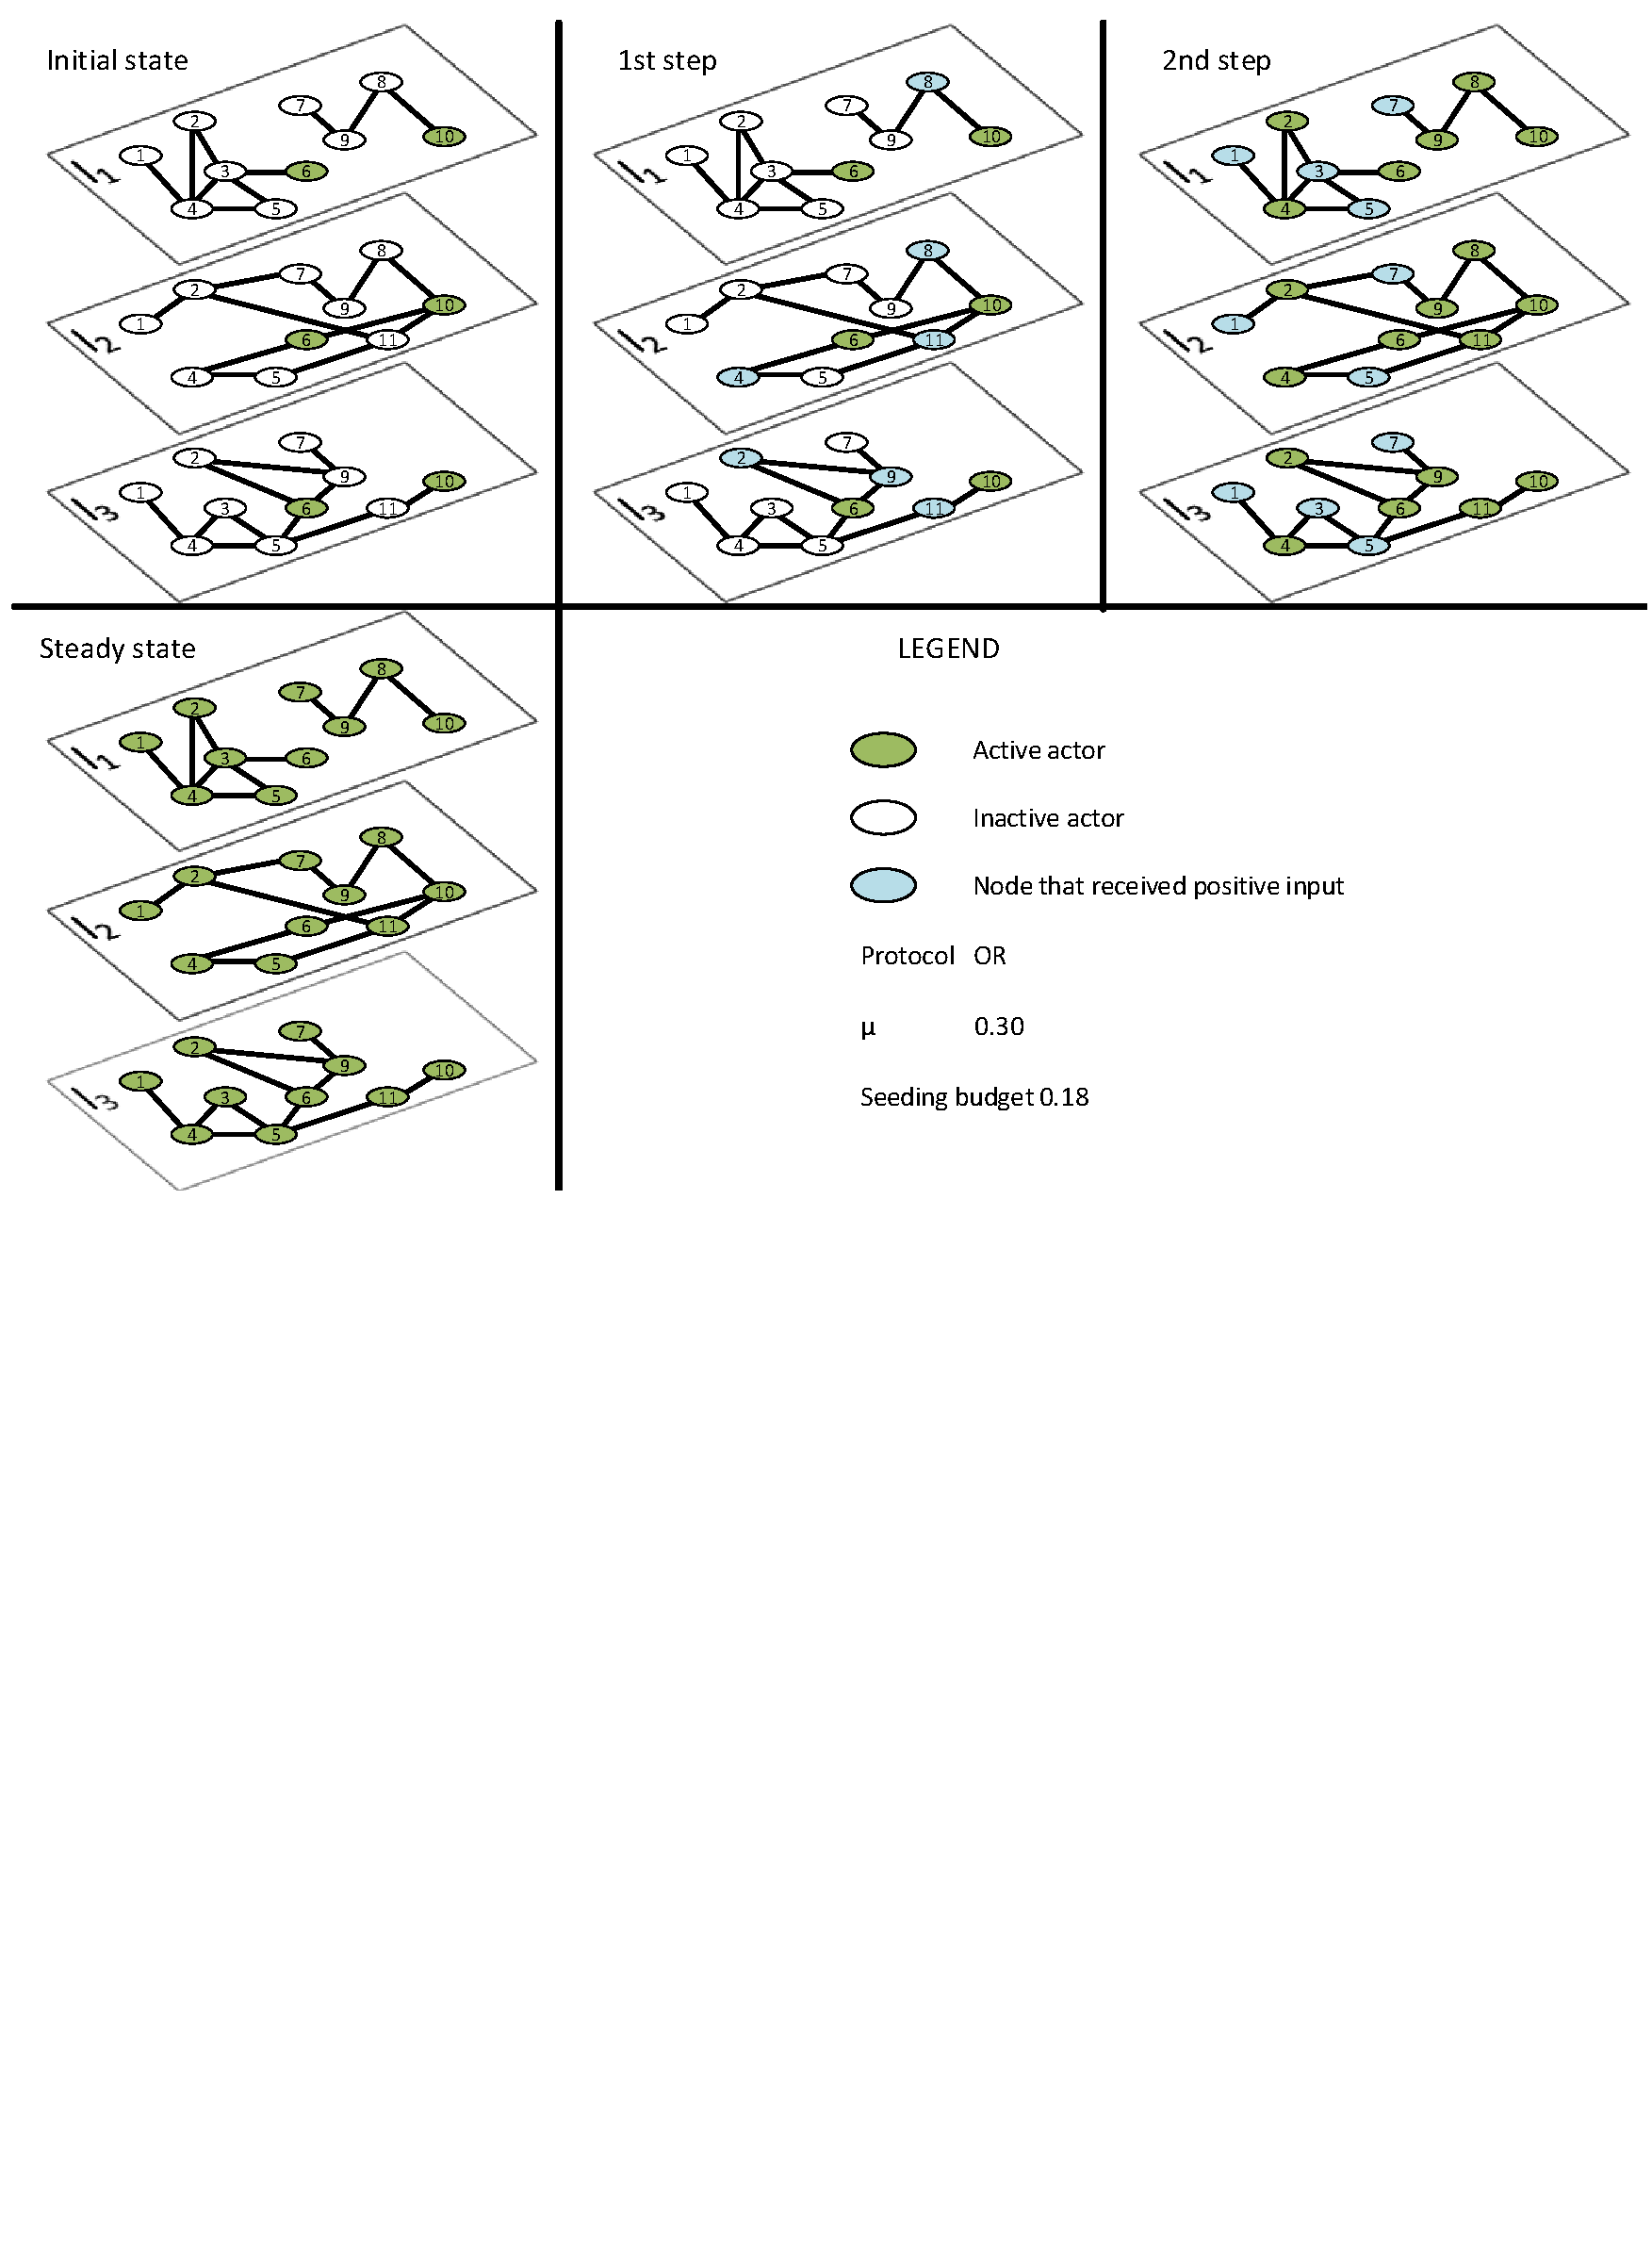
\includegraphics[width=1\linewidth]{../presentation/figures/ltm_example_or.pdf}
\end{figure}

\heading{Modelling it with \lstinline[style=py, basicstyle=\large\ttfamily]{network-diffusion}}

\begin{lstlisting}[style=py, basicstyle=\footnotesize\ttfamily]
import network_diffusion as nd

# get the graph - a medium for spreading
net = nd.mln.functions.get_toy_network_piotr()

# set actor 6 and 10 as seeds (we can use another heuristic here as well)
ac_6, ac_10 = net.get_actor(6), net.get_actor(10)
ranking_list = [ac_6, ac_10, *set(net.get_actors()).difference({ac_6, ac_10})]
seed_selector = nd.seeding.MockingActorSelector(ranking_list)
seed_quota = 100 * 2 / net.get_actors_num()

# define the model according to the given parameters
spreading_model = nd.models.MLTModel(
    seeding_budget=[100 - seed_quota, seed_quota],
    seed_selector=seed_selector,
    protocol="OR",
    mi_value=0.3,  
)

# perform the simulation that lasts four epochs
simulator = nd.Simulator(model=spreading_model, network=net)
logs = simulator.perform_propagation(n_epochs=3)

# obtain detailed logs for each actor in the form of JSON
raw_logs_json = logs.get_detailed_logs()

# or obtain aggregated logs for each of the network's layer
aggregated_logs_json = logs.get_aggragated_logs()

# or just save a summary of the experiment with all the experiment's details
logs.report(visualisation=True, path="my_experiment")
\end{lstlisting}

\heading{Outcomes}

The output logs contain a description of the network and the propagation model, a report of the
spreading for all simulated phenomena, a capture of the states of each node during the simulation,
and a brief visualisation of the propagation. They can be easily composed into subsequent data
analysis pipelines.

\begin{figure}
    \centering
    \begin{subfigure}[b]{0.36\textwidth}
        \centering
        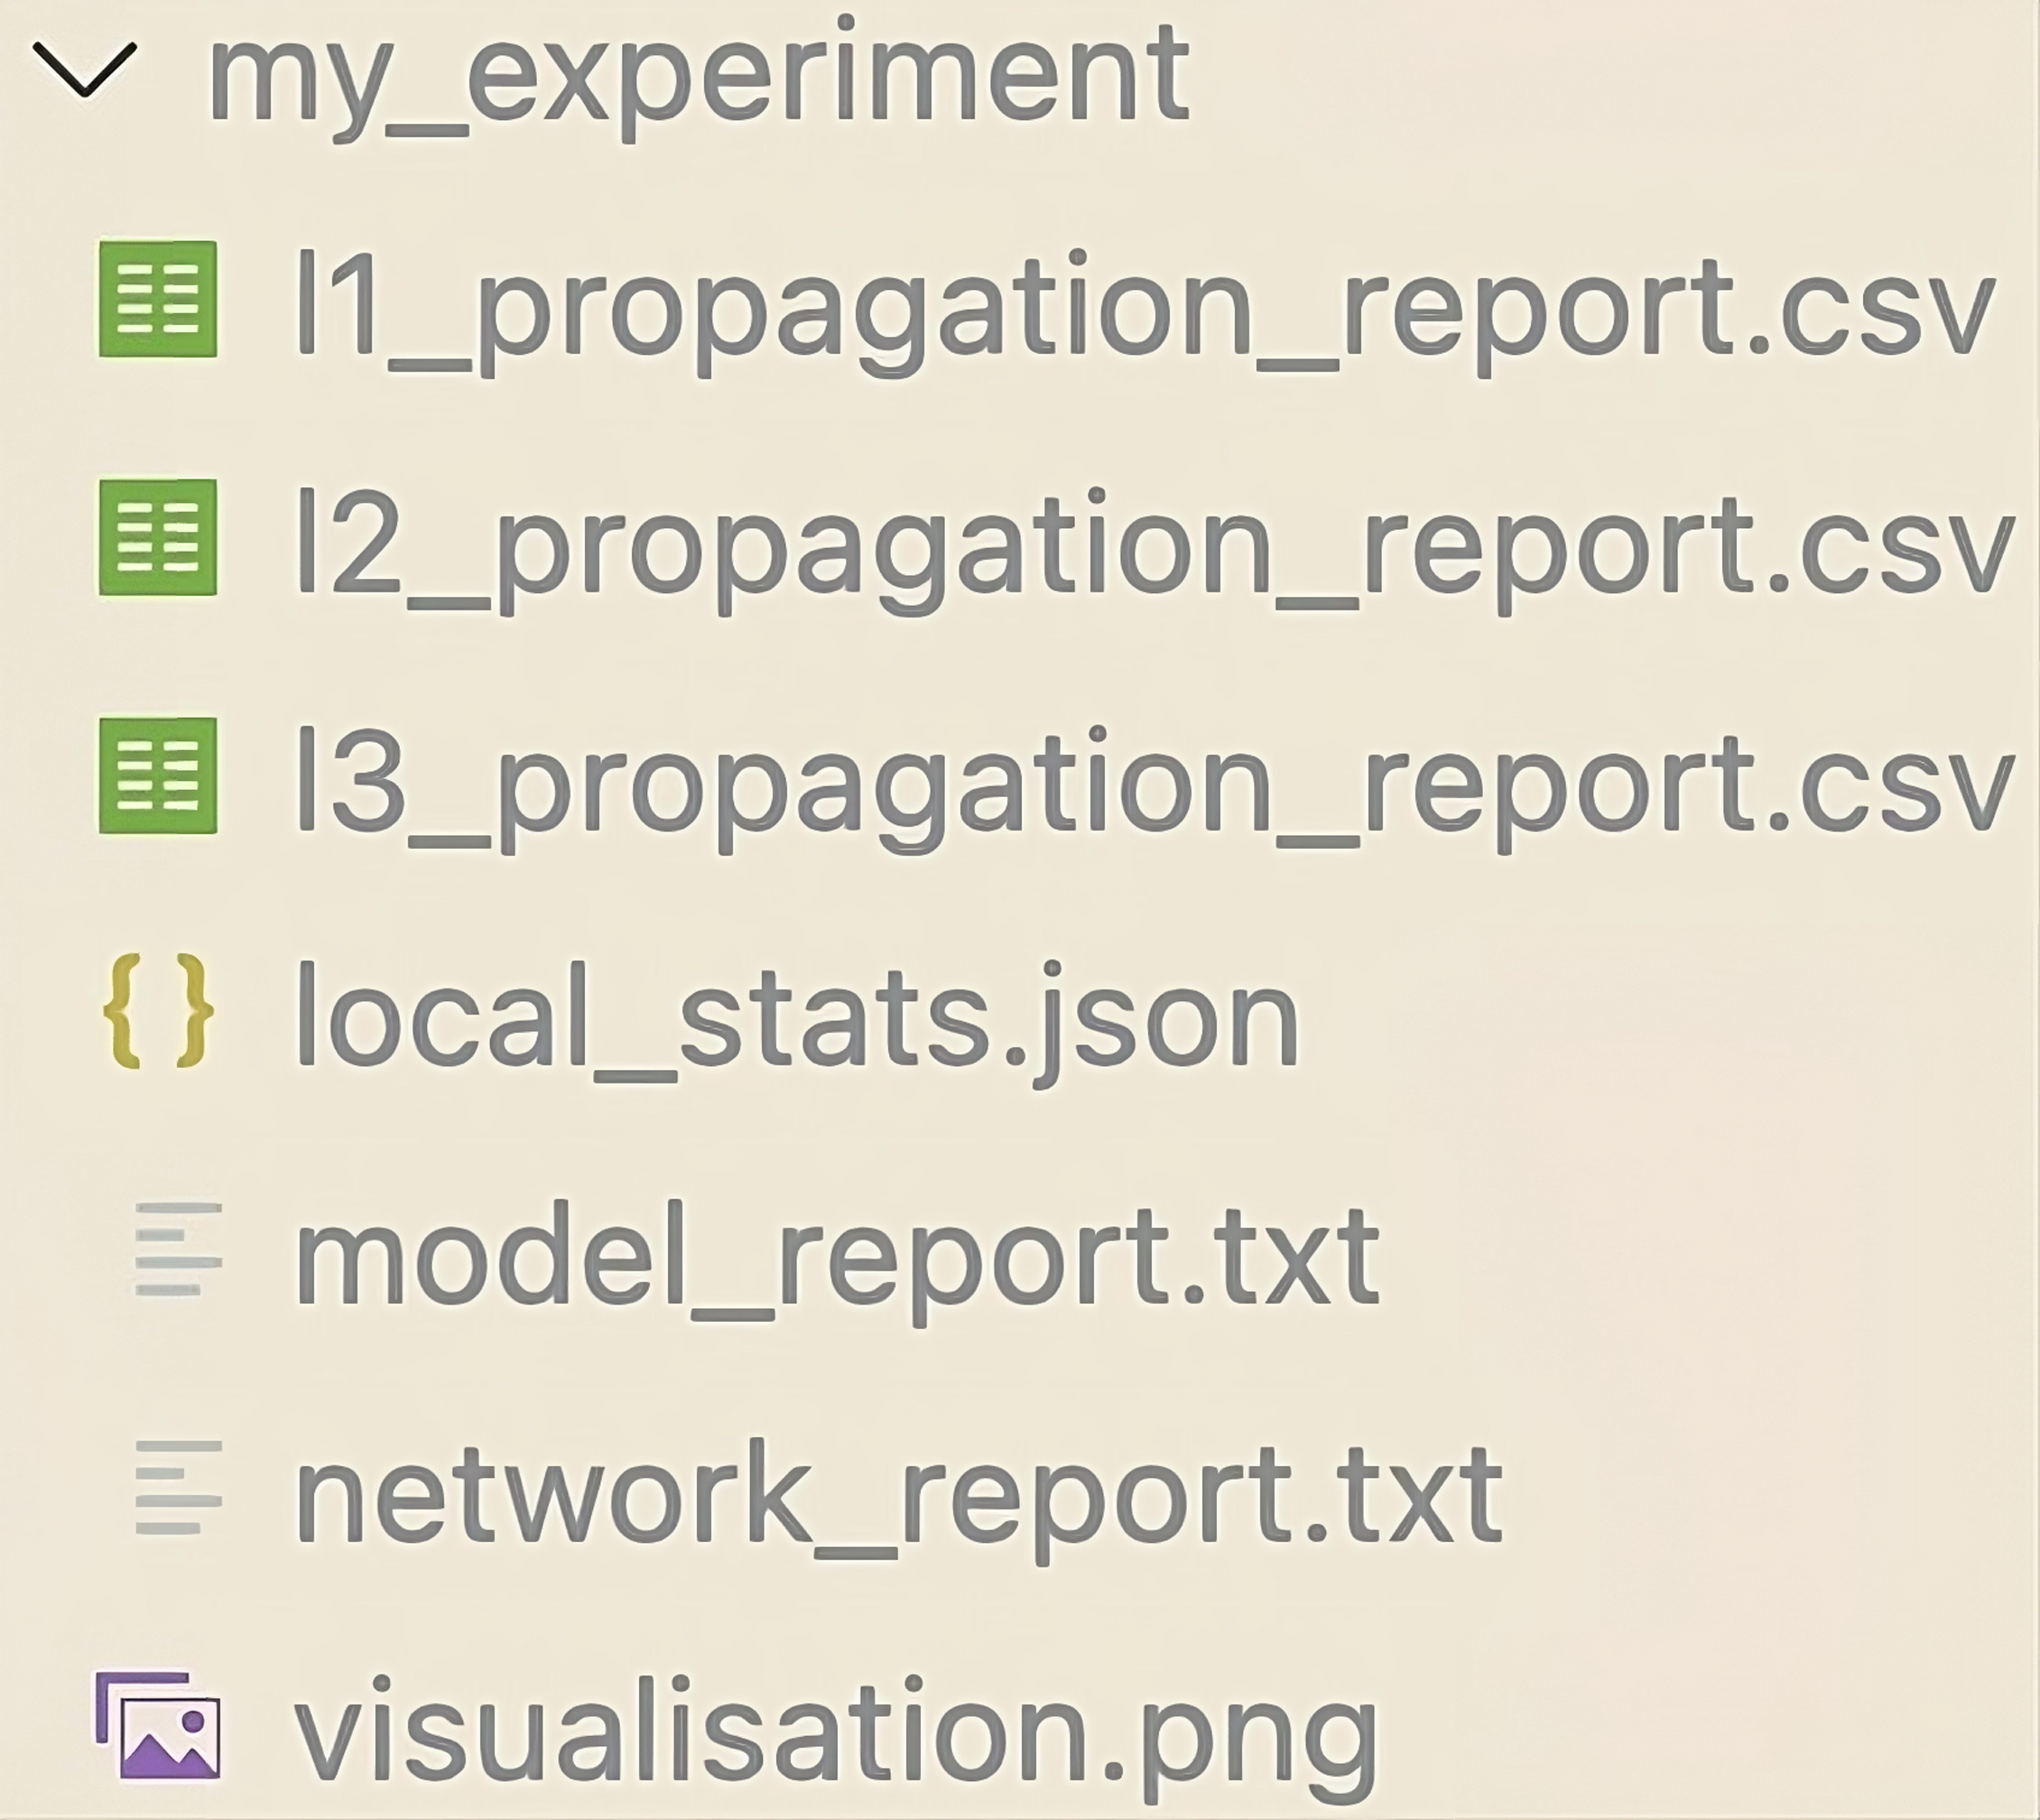
\includegraphics[width=\textwidth]{figures/output.png}
    \end{subfigure}
    \begin{subfigure}[b]{0.43\textwidth}
        \centering
        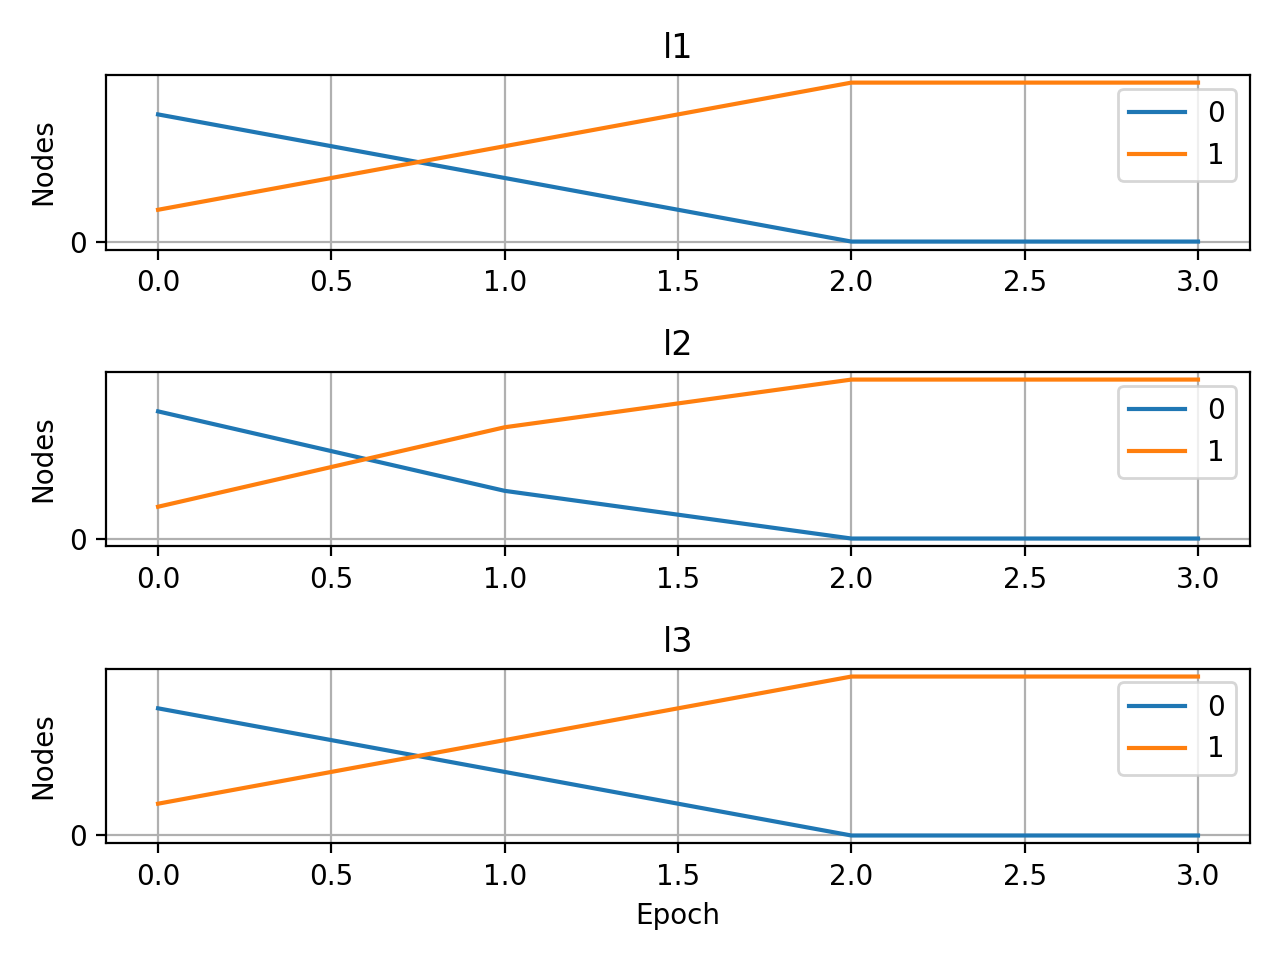
\includegraphics[width=\textwidth]{figures/visualisation.png}
    \end{subfigure}
    % \caption{kkk}
\end{figure}

\end{exampleblock}

\begin{block}{References}
    \printbibliography
\end{block}

\vspace{30em}

\end{column}
\separatorcolumn

\end{columns}
\end{frame}

\end{document}
